\subsection{Quasi-Static Examples}
\label{sec:example:3dhex8-quasistatic}

PyLith features discussed in this example:
\begin{itemize}
\item Quasi-static solution
\item Formatting timestamps of VTK output files
\item HDF5 output
\item Output of velocity field
\item Dirichlet displacement and velocity boundary conditions
\item Neumann traction boundary conditions and time-varying tractions
\item UniformDB spatial database
\item CompositeDB spatial database
\item Quasi-static fault rupture and fault creep
\item Multiple kinematic fault ruptures
\item Specifying more than one material
\item Nonlinear solver
\item Maxwell linear viscoelastic material
\item Power-law viscoelastic material
\item Drucker-Prager elastoplastic material
\item Adaptive time stepping
\end{itemize}

\subsubsection{Overview}

This set of examples describes a set of quasi-static problems for
PyLith. These quasi-static problems primarily demonstrate the usage
of time-dependent boundary conditions and fault slip, as well as different
rheologies. Some of the examples also demonstrate the usage of the
nonlinear solver, which is required by the nonlinear rheologies (power-law
viscoelastic and Drucker-Prager elastoplastic). Some of the examples
also demonstrate the usage of HDF5 output, which is an alternative
to the default VTK output. All of the examples are contained in the
directory \filename{examples/3d/hex8}, and the corresponding \filename{cfg}
files are \filename{step04.cfg}, \filename{step05.cfg}, \filename{step06.cfg},
\filename{step07.cfg}, \filename{step08.cfg}, and \filename{step09.cfg}.
Run the examples as follows:
\begin{shell}
# Step04
$ pylith step04.cfg

# Step05
$ pylith step05.cfg

# Step06
$ pylith step06.cfg

# Step07
$ pylith step07.cfg

# Step08
$ pylith step08.cfg

# Step09
$ pylith step09.cfg
\end{shell}
This will cause PyLith to read the default parameters in \filename{pylithapp.cfg},
and then override or augment them with the additional parameters in
the \filename{stepXX.cfg} file. Each \filename{cfg} file is extensively
documented, to provide detailed information on the various parameters.


\subsubsection{Step04 - Pure Dirichlet Velocity Boundary Conditions}

The \filename{step04.cfg} file defines a problem with x-displacements
fixed at zero on the positive and negative x-faces while velocity
boundary conditions are applied in the y-directions on the same faces,
yielding a left-lateral sense of movement. The bottom (negative z)
boundary is held fixed in the z-direction. We also use a Maxwell viscoelastic
material for the lower crust, and the simulation is run for 200 years
using a constant time-step size of 20 years. The default time stepping
behavior is \object{TimeStepUniform}. We retain that behavior for
this problem and provide the total simulation time and the time-step
size:
\begin{cfg}[Excerpt from \filename{step04.cfg}]
# Change the total simulation time to 200 years, and use a constant time
# step size of 20 years.
<h>[pylithapp.timedependent.implicit.time_step]<.h>
<p>total_time</p> = 200.0*year
<p>dt</p> = 20.0*year 
\end{cfg}
We then change the material type of the lower crust, provide a spatial
database from which to obtain the material properties (using the default
\object{SimpleDB}), and request additional output information for
the material:
\begin{cfg}[Excerpt from \filename{step04.cfg}]
# Change material type of lower crust to Maxwell viscoelastic.
<h>[pylithapp.timedependent]</h>
<f>materials.lower_crust</f> = pylith.materials.MaxwellIsotropic3D

# Provide a spatial database from which to obtain property values.
# Since there are additional properties and state variables for the Maxwell
# model, we explicitly request that they be output. Properties are named in
# cell_info_fields and state variables are named in cell_data_fields.
<h>[pylithapp.timedependent.materials.lower_crust]</h>
<p>db_properties.iohandler.filename</p> = spatialdb/mat_maxwell.spatialdb
<p>output.cell_info_fields</p> = [density, mu, lambda, maxwell_time]
<p>output.cell_data_fields</p> = [total_strain, stress, viscous_strain]
\end{cfg}
Note that the default \property{output.cell\_info\_fields} are those
corresponding to an elastic material (\texttt{density}, \texttt{mu},
\texttt{lambda}), and the default \property{output.cell\_data\_fields}
are \texttt{total\_strain} and \texttt{stress}. For materials other
than elastic, there are generally additional material properties and
state variables, and the appropriate additional fields must be specifically
requested for each material type.

This example has no displacements in the elastic solution (t = 0),
so we retain the default \object{ZeroDispDB} for all instances of
\facility{db\_initial}. To apply the velocity boundary conditions, we
must specify \facility{db\_rate}, which is zero by default. We use a
\object{UniformDB} to assign the velocities:
\begin{cfg}[Excerpt from \filename{step04.cfg}]
# Boundary condition on +x face
<h>[pylithapp.timedependent.bc.x_pos]</h>
<p>bc_dof</p> = [0, 1]
<p>label</p> = face_xpos
<p>db_initial.label</p> = Dirichlet BC on +x
<f>db_rate</f> = spatialdata.spatialdb.UniformDB
<p>db_rate.label</p> = Dirichlet rate BC on +x
<p>db_rate.values</p> = [displacement-rate-x, displacement-rate-y, rate-start-time]
<p>db_rate.data</p> = [0.0*cm/year, 1.0*cm/year, 0.0*year]

# Boundary condition on -x face
<h>[pylithapp.timedependent.bc.x_neg]</h>
<p>bc_dof</p> = [0, 1]
<p>label</p> = face_xneg
<p>db_initial.label</p> = Dirichlet BC on -x
<f>db_rate</f> = spatialdata.spatialdb.UniformDB
<p>db_rate.label</p> = Dirichlet rate BC on +x
<p>db_rate.values</p> = [displacement-rate-x, displacement-rate-y, rate-start-time]
<p>db_rate.data</p> = [0.0*cm/year, -1.0*cm/year, 0.0*year]
\end{cfg}
Note that \facility{db\_rate} requires a start time, which allows the
condition to be applied at any time during the simulation. For this
example, we start the velocity boundary conditions at t = 0.

Finally, we must provide information on VTK output. This is slightly
more complicated than the static case, because we must decide the
frequency with which output occurs for each output manager. We also
assign a more user-friendly format to the output file time stamp,
and we request that the time stamp is in units of 1 year (rather than
the default value of seconds):
\begin{cfg}[Excerpt from \filename{step04.cfg}]
# Give basename for VTK domain output of solution over domain.
<h>[pylithapp.problem.formulation.output.domain]</h>
# We specify that output occurs in terms of a given time frequency, and
# ask for output every 40 years. The time stamps of the output files are
# in years (rather than the default of seconds), and we give a format for
# the time stamp.
<p>output_freq</p> = time_step
<p>time_step</p> = 40.0*year
<p>writer.filename</p> = output/step04.vtk
<p>writer.time_format</p> = \%04.0f
<p>writer.time_constant</p> = 1.0*year

# Give basename for VTK domain output of solution over ground surface.
<h>[pylithapp.problem.formulation.output.subdomain]</h>
<p>label</p> = face_zpos ; Name of nodeset for ground surface
# We keep the default output frequency behavior (skip every n steps), and
# ask to skip 0 steps between output, so that we get output every time step.
<p>skip</p> = 0
<p>writer.filename</p> = output/step04-groundsurf.vtk
<p>writer.time_format</p> = %04.0f
<p>writer.time_constant</p> = 1.0*year
\end{cfg}
We provide similar output information for the two materials (\facility{upper\_crust}
and \facility{lower\_crust}). Note that for the domain output, we requested
output in terms of a given time frequency, while for the subdomain
we requested output in terms of number of time steps. When we have
run the simulation, the output VTK files will be contained in \filename{examples/3d/hex8/output}
(all with a prefix of \filename{step04}). Results using ParaView are
shown in Figure \vref{fig:example:3dhex8:step04:displacement}.

\begin{figure}
  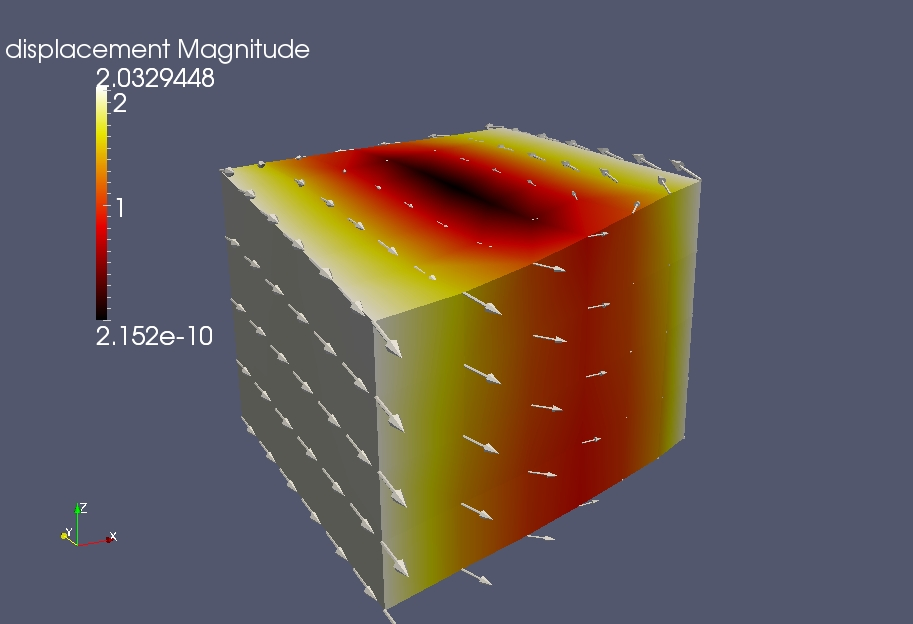
\includegraphics[width=10cm]{examples/figs/3dhex8_step04-displ-t200}
  \caption{Displacement field for example step04 at t = 200 years
    visualized using ParaView. The mesh has been distorted by the
    computed displacements (magnified by 500), and the vectors show
    the computed displacements.}
  \label{fig:example:3dhex8:step04:displacement}
\end{figure}


\subsubsection{Step05 - Time-Varying Dirichlet and Neumann Boundary Conditions}

The \filename{step05.cfg} file describes a problem with time-varying
Dirichlet and Neumann boundary conditions. The example is similar
to example step04, with a few important differences:
\begin{itemize}
\item The Dirichlet boundary conditions on the negative x-face include an
  initial displacement (applied in the elastic solution), as well as
  a constant velocity.
\item Neumann (traction) boundary conditions are applied in the negative
  x-direction on the positive x-face, giving a compressive stress. An
  initial traction is applied in the elastic solution, and then at t
  = 100 years it begins decreasing linearly until it reaches zero at
  the end of the simulation (t = 200 years).
\end{itemize}
We again use a Maxwell viscoelastic material for the lower crust.

For the boundary conditions, we must first change the boundary condition
type for the positive x-face from the default Dirichlet to Neumann:
\begin{cfg}[Excerpt from \filename{step05.cfg}]
# +x face -- first change bc type to Neumann
<h>[pylithapp.timedependent.bc]</h>
<f>x_pos</f> = pylith.bc.Neumann 
\end{cfg}
We provide quadrature information for this face as we did for example
step02. We then use a \object{UniformDB} for both the initial tractions
as well as the traction rates. We provide a start time of 100 years
for the traction rates, and use a rate of 0.01 MPa/year, so that by
the end of 200 years we have completely cancelled the initial traction
of -1 MPa:
\begin{cfg}[Excerpt from \filename{step05.cfg}]
<h>[pylithapp.timedependent.bc.x_pos]</h>
# First specify a UniformDB for the initial tractions, along with the values.
<f>db_initial</f> = spatialdata.spatialdb.UniformDB
<p>db_initial.label</p> = Neumann BC on +x
<p>db_initial.values</p> = [traction-shear-horiz, traction-shear-vert, traction-normal]
<p>db_initial.data</p> = [0.0*MPa, 0.0*MPa, -1.0*MPa]

# Provide information on traction rates.
<f>db_rate</f> = spatialdata.spatialdb.UniformDB
<p>db_rate.label</p> = Neumann rate BC on +x
<p>db_rate.values</p> = [traction-rate-shear-horiz, traction-rate-shear-vert, traction-rate-normal,rate-start-time]
<p>db_rate.data</p> = [0.0*MPa/year, 0.0*MPa/year, 0.01*MPa/year, 100.0*year]
\end{cfg}
The boundary conditions on the negative x-face are analogous, but
we are instead using Dirichlet boundary conditions, and the initial
displacement is in the same direction as the applied velocities:
\begin{cfg}[Excerpt from \filename{step05.cfg}]
# -x face
<h>[pylithapp.timedependent.bc.x_neg]</h>
<p>bc_dof<p> = [0, 1]
<p>label</p> = face_xneg

# Initial displacements.
<f>db_initial</f> = spatialdata.spatialdb.UniformDB
<p>db_initial.label</p> = Dirichlet BC on -x
<p>db_initial.values</p> = [displacement-x, displacement-y]
<p>db_initial.data</p> = [0.0*cm, -0.5*cm]

# Velocities.
<f>db_rate</f> = spatialdata.spatialdb.UniformDB
<p>db_rate.label</p> = Dirichlet rate BC on -x
<p>db_rate.values</p> = [displacement-rate-x,displacement-rate-y,rate-start-time]
<p>db_rate.data</p> = [0.0*cm/year, -1.0*cm/year, 0.0*year]
\end{cfg}
The boundary conditions on the negative z-face are supplied in the
same manner as for example step04. When we have run the simulation,
the output VTK files will be contained in \filename{examples/3d/hex8/output}
(all with a prefix of \filename{step05}). Results using ParaView are
shown in Figure \vref{fig:example:3dhex8:step05:displacement}.

\begin{figure}
  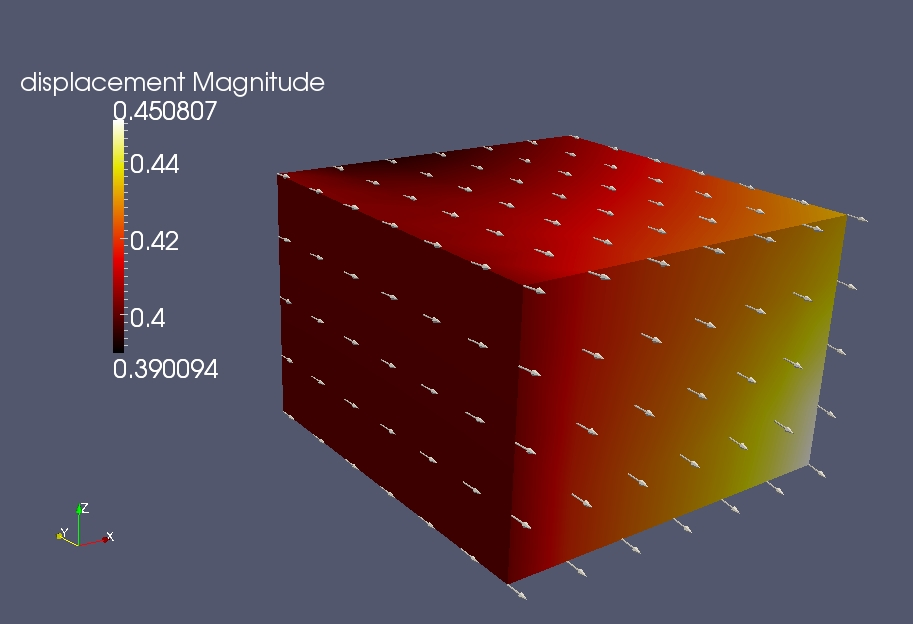
\includegraphics[width=10cm]{examples/figs/3dhex8_step05-displ-t40}
  \caption{Displacement field for example step05 at t = 40 years visualized using
    ParaView. The mesh has been distorted by the computed displacements
    (magnified by 500), and the vectors show the computed displacements.}
  \label{fig:example:3dhex8:step05:displacement}
\end{figure}


\subsubsection{Step06 - Dirichlet Boundary Conditions with Time-Dependent Kinematic Fault Slip}

The \filename{step06.cfg} file defines a problem with Dirichlet (displacement)
boundary conditions corresponding to zero x- and y-displacements applied
on the negative and positive x-faces and a vertical fault that includes
multiple earthquake ruptures as well as steady fault creep. The upper
(locked) portion of the fault has 4 m of left-lateral slip every 200
years, while the lower (creeping) portion of the fault slips at a
steady rate of 2 cm/year. The problem bears some similarity to the
strike-slip fault model of Savage and Prescott \cite{Savage:Prescott:1978},
except that the fault creep extends through the viscoelastic portion
of the domain, and the far-field displacement boundary conditions
are held fixed.

In this example and the remainder of the examples in this section,
we change the time stepping behavior from the default \object{TimeStepUniform}
to \object{TimeStepAdapt}. For adaptive time stepping, we provide
the maximum permissible time-step size, along with a stability factor.
The stability factor controls the time-step size relative to the stable
time-step size provided by the different materials in the model. A
\property{stability\_factor} of 1.0 means we should use the stable time-step
size, while a \property{stability\_factor} greater than 1.0 means we
want to use a smaller time-step size. A \property{stability\_factor}
less than 1.0 allows time-step sizes greater than the stable time-step
size, which may provide inaccurate results. The adaptive time stepping
information is provided as:
\begin{cfg}[Excerpt from \filename{step06.cfg}]
# Change time stepping algorithm from uniform time step, to adaptive
# time stepping.
<f>time_step</f> = pylith.problems.TimeStepAdapt

# Change the total simulation time to 700 years, and set the maximum time
# step size to 10 years.
<h>[pylithapp.timedependent.implicit.time_step]</h>
<p>total_time</p> = 700.0*year
<p>max_dt</p> = 10.0*year
<p>stability_factor</p> = 1.0 ; use time step equal to stable value from materials
\end{cfg}
In this example and the remainder of the examples in this section,
we also make use of HDF5 output rather than the default VTK output.
HDF5 output is a new feature beginning with PyLith version 1.6, and
it is much more efficient with the additional advantage that multiple
time steps can be contained in a single file. PyLith also produces
Xdmf files describing the contents of the HDF5 files, which allows
the files to be read easily by applications such as ParaView. Since
VTK output is still the default, we must change the value from the
default. Also note that the filename suffix is \filename{h5}:
\begin{cfg}[Excerpt from \filename{step06.cfg}]
# Give basename for output of solution over domain.
<h>[pylithapp.problem.formulation.output.domain]</h>
# We specify that output occurs in terms of a given time frequency, and
# ask for output every 50 years.
<p>output_freq</p> = time_step
<p>time_step</p> = 50.0*year

# We are using HDF5 output so we must change the default writer.
<f>writer</f> = pylith.meshio.DataWriterHDF5
<p>writer.filename</p> = output/step06.h5  
\end{cfg}
Note that we no longer need the \property{writer.time\_format} or
\property{writer.time\_constant} properties, since all time steps are
contained in a single file. The HDF5 writer does not have these
properties, so if we attempt to define them an error will result.

We also set the writer for other output as well, since it is not the
default. For subdomain output we use:
\begin{cfg}[Excerpt from \filename{step06.cfg}]
# Give basename for output of solution over ground surface.
<h>[pylithapp.problem.formulation.output.subdomain]</h>
# Name of nodeset for ground surface.
<p>label</p> = face_zpos

# We keep the default output frequency behavior (skip every n steps), and
# ask to skip 0 steps between output, so that we get output every time step.
# We again switch the writer to produce HDF5 output.
<p>skip</p> = 0
<f>writer</f> = pylith.meshio.DataWriterHDF5
<p>writer.filename</p> = output/step06-groundsurf.h5  

# Fault output
<h>[pylithapp.problem.interfaces.fault.output]</h>
# We keep the default output frequency behavior (skip every n steps), and
# ask to skip 0 steps between output, so that we get output every time step.
# We again switch the writer to produce HDF5 output.
<p>skip</p> = 0
<f>writer</f> = pylith.meshio.DataWriterHDF5
<p>writer.filename</p> = output/step06-fault.h5
\end{cfg}
Due to the simplicity of the boundary conditions, we are able to use
the default \object{ZeroDispBC} for the positive and negative x-faces,
as well as the negative z-face. As for example step03, we define a
fault interface, we identify the nodeset corresponding to the fault,
and we provide quadrature information for the fault. We then define
an array of earthquake sources and provide an origin time for each:
\begin{cfg}[Excerpt from \filename{step06.cfg}]
<h>[pylithapp.timedependent.interfaces.fault]</h>
# Set earthquake sources to an array consisting of creep and 3 ruptures.
<f>eq_srcs</f> = [creep, one, two, three]
<p>eq_srcs.creep.origin_time</p> = 00.0*year
<p>eq_srcs.one.origin_time</p> = 200.0*year
<p>eq_srcs.two.origin_time</p> = 400.0*year
<p>eq_srcs.three.origin_time</p> = 600.0*year
\end{cfg}
Note that the creep begins at t = 0 years, while the ruptures (\facility{one},
\facility{two}, \facility{three}) occur at regular intervals of 200 years.
We retain the default \object{StepSlipFn} for the ruptures. Each of
the ruptures has the same amount of slip, and slip occurs simultaneously
for the entire rupture region, so we can use the same \object{SimpleDB}
files providing slip and slip time for each rupture:
\begin{cfg}[Excerpt from \filename{step06.cfg}]
# Define slip and origin time for first rupture.
<h>[pylithapp.timedependent.interfaces.fault.eq_srcs.one.slip_function]</h>
<p>slip.iohandler.filename</p> = spatialdb/finalslip_rupture.spatialdb
<p>slip_time.iohandler.filename</p> = spatialdb/sliptime.spatialdb

# Define slip and origin time for second rupture.
<h>[pylithapp.timedependent.interfaces.fault.eq_srcs.two.slip_function]</h>
<p>slip.iohandler.filename</p> = spatialdb/finalslip_rupture.spatialdb
<p>slip_time.iohandler.filename</p> = spatialdb/sliptime.spatialdb

# Define slip and origin time for third rupture.
<h>[pylithapp.timedependent.interfaces.fault.eq_srcs.three.slip_function]</h>
<p>slip.iohandler.filename</p> = spatialdb/finalslip_rupture.spatialdb
<p>slip_time.iohandler.filename</p> = spatialdb/sliptime.spatialdb
\end{cfg}
For the creep source, we change the slip function to \object{ConstRateSlipFn},
and we use a \object{SimpleDB} for both the slip time and the slip
rate:
\begin{cfg}[Excerpt from \filename{step06.cfg}]
# Define slip rate and origin time for fault creep.
<h>[pylithapp.timedependent.interfaces.fault.eq_srcs.creep]</h>
<f>slip_function</f> = pylith.faults.ConstRateSlipFn
<p>slip_function.slip_rate.iohandler.filename</p> = spatialdb/sliprate_creep.spatialdb
<p>slip_function.slip_time.iohandler.filename</p> = spatialdb/sliptime.spatialdb
\end{cfg}
For all earthquake sources we provide both an \property{origin\_time}
and a \property{slip\_function.slip\_time}. The first provides the starting
time for the entire earthquake source, while the second provides any
spatial variation in the slip time with respect to the \property{origin\_time}
(if any). Since there are multiple earthquake sources of different
types, there are a number of additional fault information fields available
for output. We add these additional fields' output to the fault information
file:
\begin{cfg}[Excerpt from \filename{step06.cfg}]
<h>[pylithapp.timedependent.interfaces.fault]</h>
<p>output.vertex_info_fields</p> = [normal_dir, strike_dir, dip_dir, final_slip_creep, \
  final_slip_one, final_slip_two, final_slip_three, slip_time_creep, slip_time_one, \
  slip_time_two, slip_time_three]
\end{cfg}
This additional information will be contained in file \filename{step06-fault\_info.h5}.
It will contain final slip information for each earthquake source
along with slip time information. When we have run the simulation,
the output HDF5 and Xdmf files will be contained in \filename{examples/3d/hex8/output}
(all with a prefix of \filename{step06}). To open the files in ParaView,
the Xdmf (\filename{xmf}) files should be opened, as these files describe
the HDF5 data structure. Results using ParaView are shown in Figure
\vref{fig:example:3dhex8:step06:displacement}.

\begin{figure}
  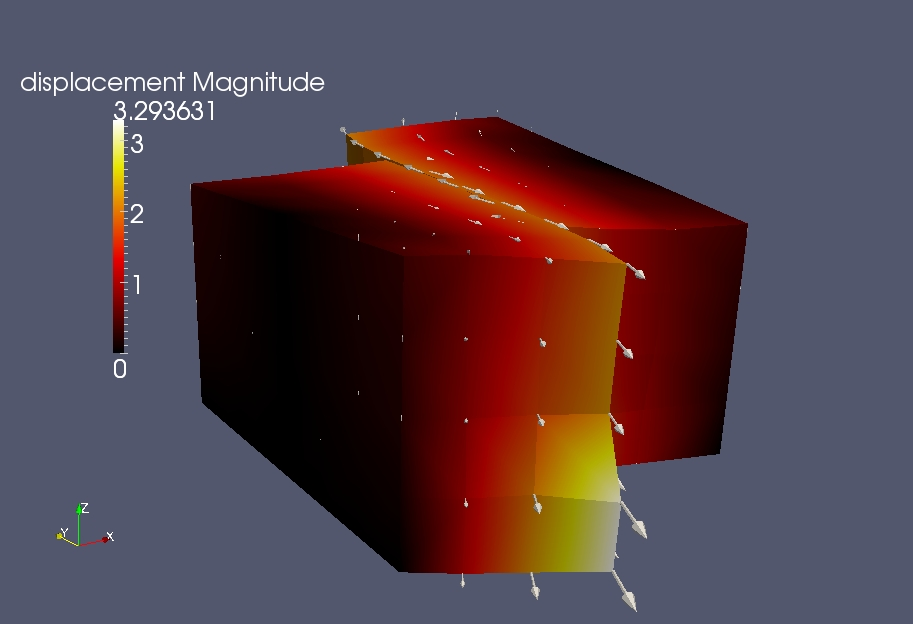
\includegraphics[width=10cm]{examples/figs/3dhex8_step06-displ-t300}
  \caption{Displacement field for example step06 at t = 300 years visualized
    using ParaView. The mesh has been distorted by the computed displacements
    (magnified by 500), and the vectors show the computed displacements.}
  \label{fig:example:3dhex8:step06:displacement}
\end{figure}


\subsubsection{Step07 - Dirichlet Velocity Boundary Conditions with Time-Dependent Kinematic Fault Slip}

In step07 we add velocity boundary conditions in the positive and
negative y-directions on the positive and negative x-faces, so that
the external boundaries keep pace with the average fault slip. This
problem is nearly identical to the strike-slip fault model of Savage
and Prescott \cite{Savage:Prescott:1978}, except that the fault creep
extends through the viscoelastic portion of the domain.

We use the default \object{ZeroDispBC} for the initial displacements
on the positive and negative x-faces, as well as the negative z-face.
For the velocities on the positive and negative x-faces, we use a
\object{UniformDB}:
\begin{cfg}`w
# Boundary condition on +x face
[pylithapp.timedependent.bc.x_pos]
<p>bc_dof</p> = [0, 1]
<p>label</p> = face_xpos
<p>db_initial.label</p> = Dirichlet BC on +x
<f>db_rate</f> = spatialdata.spatialdb.UniformDB
<p>db_rate.label</p> = Dirichlet rate BC on +x
<p>db_rate.values</p> = [displacement-rate-x, displacement-rate-y, rate-start-time]
<p>db_rate.data</p> = [0.0*cm/year, 1.0*cm/year, 0.0*year]

# Boundary condition on -x face
<h>[pylithapp.timedependent.bc.x_neg]</h>
<p>bc_dof</p> = [0, 1]
<p>label</p> = face_xneg
<p>db_initial.label</p> = Dirichlet BC on -x
<f>db_rate</f> = spatialdata.spatialdb.UniformDB
<p>db_rate.label</p> = Dirichlet rate BC on +x
<p>db_rate.values</p> = [displacement-rate-x, displacement-rate-y, rate-start-time]
<p>db_rate.data</p> = [0.0*cm/year, -1.0*cm/year, 0.0*year]
\end{cfg}
The fault definition information is identical to example \filename{step06}.
In previous examples, we have just used the default output for the
domain and subdomain (ground surface), which includes the displacements.
In many cases, it is also useful to include the velocities. PyLith
provides this information, computing the velocities for the current
time step as the difference between the current displacements and
the displacements from the previous time step, divided by the time-step
size. This is more accurate than computing the velocities from the
displacement field output that has been decimated in time. We can
obtain this information by explicitly requesting it in \property{vertex\_data\_fields}:
\begin{cfg}[Excerpt from \filename{step07.cfg}]
# Give basename for output of solution over domain.
<h>[pylithapp.problem.formulation.output.domain]</h>
# We specify that output occurs in terms of a given time frequency, and
# ask for output every 50 years.
# We also request velocity output in addition to displacements.
<p>vertex_data_fields</p> = [displacement, velocity]
<p>output_freq</p> = time_step
<p>time_step</p> = 50.0*year

# We are using HDF5 output so we must change the default writer.
<f>writer</f> = pylith.meshio.DataWriterHDF5
<p>writer.filename</p> = output/step07.h5

# Give basename for output of solution over ground surface.
<h>[pylithapp.problem.formulation.output.subdomain]</h>
# Name of nodeset for ground surface.
<p>label</p> = face_zpos

# We also request velocity output in addition to displacements.
<p>vertex_data_fields</p> = [displacement, velocity]
# We keep the default output frequency behavior (skip every n steps), and
# ask to skip 0 steps between output, so that we get output every time step.
<p>skip</p> = 0

# We again switch the writer to produce HDF5 output.
<f>writer</f> = pylith.meshio.DataWriterHDF5
<p>writer.filename</p> = output/step07-groundsurf.h5
\end{cfg}
When we have run the simulation, the output HDF5 and Xdmf files will
be contained in \filename{examples/3d/hex8/output} (all with a prefix
of \filename{step07}). As for example step06, make sure to open the
\filename{xmf} files rather than the \filename{h5} files. Results using
ParaView are shown in Figure \vref{fig:example:3dhex8:step07:displacement}.

\begin{figure}
  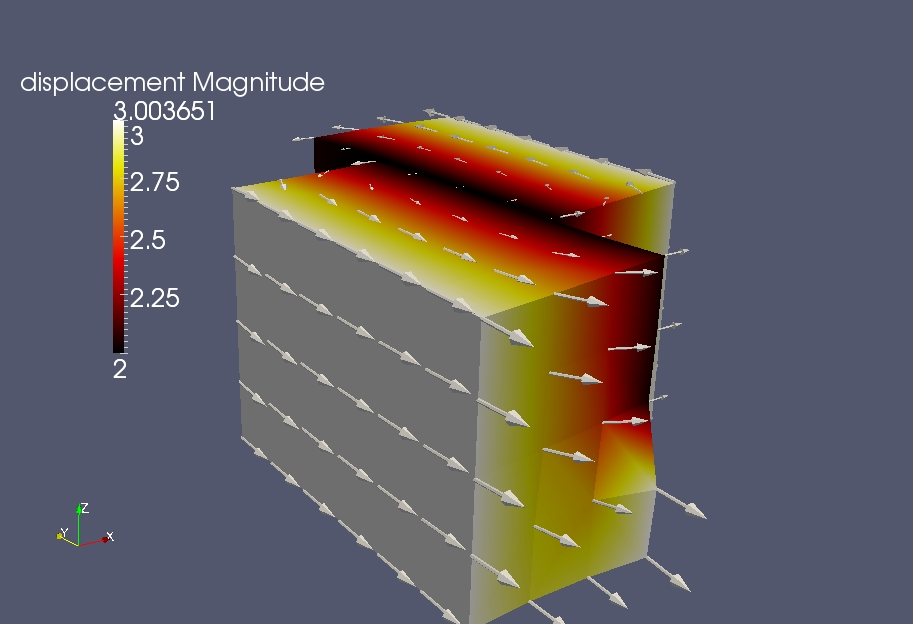
\includegraphics[width=10cm]{examples/figs/3dhex8_step07-displ-vel-t300}
  \caption{Displacement field (color contours) and velocity field (vectors) for
    example step07 at t = 300 years visualized using ParaView. The mesh
    has been distorted by the computed displacements (magnified by 500),
    and the vectors show the computed velocities.}
  \label{fig:example:3dhex8:step07:displacement}
\end{figure}


\subsubsection{Step08 - Dirichlet Velocity Boundary Conditions with Time-Dependent Kinematic Fault Slip and Power-Law Rheology}
\label{sec:example:3dhex8:step08}

The \filename{step08.cfg} file defines a problem that is identical to
example step07, except the the lower crust is composed of a power-law
viscoelastic material. Since the material behavior is now nonlinear,
we must use the nonlinear solver:
\begin{cfg}[Excerpt from \filename{step08.cfg}]
<h>[pylithapp.timedependent]</h>
# For this problem we must switch to a nonlinear solver.
<f>implicit.solver</f> = pylith.problems.SolverNonlinear
\end{cfg}
Although we have not discussed the PyLith PETSc settings previously,
note that the use of the nonlinear solver may require additional options
if we wish to override the defaults. These settings are contained
in \filename{pylithapp.cfg}:
\begin{cfg}[Excerpt from \filename{step08.cfg}]
<h>[pylithapp.petsc]</h>
# Nonlinear solver monitoring options.
<p>snes_rtol</p> = 1.0e-8
<p>snes_atol</p> = 1.0e-12
<p>snes_max_it</p> = 100
<p>snes_monitor</p> = true
<p>snes_view</p> = true
<p>snes_converged_reason</p> = true
\end{cfg}
These settings are ignored unless we are using the nonlinear solver.

When setting the physical properties for the power-law material in
PyLith, the parameters (see Section
\vref{sec:materials:formulation:powerlaw}) do not generally correspond
to the values provided in laboratory results.  PyLith includes a
utility code, \filename{powerlaw\_gendb.py}, to simplify the process
of using laboratory results with PyLith. This utility code is
installed in the same location as PyLith. An example of how to use it
is in \filename{examples/3d/hex8/spatialdb/powerlaw}. The user must
provide a spatial database defining the spatial distribution of
laboratory-derived parameters (contained in
\filename{powerlaw\_params.spatialdb}), another spatial database
defining the temperature field in degrees K (contained in
\filename{temperature.spatialdb}), and a set of points for which
values are desired (\filename{powerlaw\_points.txt}).  The parameters
for the code are defined in \filename{powerlaw\_gendb.cfg}.  The
properties expected by PyLith are \texttt{reference\_strain\_rate},
\texttt{reference\_stress}, and \texttt{power\_law\_exponent}. The
user must specify either \texttt{reference\_strain\_rate} or
\texttt{reference\_stress} so that \filename{powerlaw\_gendb.py} can
compute the other property.  Default values of 1.0e-6 1/s and 1 MPa
are provided. In this example, the same database was used for all
parameters, and a separate database was used to define the temperature
distribution. In practice, the user can provide any desired thermal
model to provide the spatial database for the temperature. In this
example, a simple 1D (vertically-varying) distribution was used. The
utility code can be used by simply executing it from the
\filename{examples/3d/hex8/spatialdb/powerlaw} directory:
\begin{shell}
$ powerlaw_gendb.py
\end{shell}
This code will automatically read the parameters in \filename{powerlaw\_gendb.cfg}
in creating the file \filename{examples/3d/hex8/spatialdb/mat\_powerlaw.spatialdb}.

We first change the material type of the lower crust to \object{PowerLaw3D}:
\begin{cfg}[Excerpt from \filename{step08.cfg}]
# Change material type of lower crust to power-law viscoelastic.
<h>[pylithapp.timedependent]</h>
<f>materials.lower_crust</f> = pylith.materials.PowerLaw3D
\end{cfg}
In many cases, it is useful to obtain the material properties from two
different sources. For example, the elastic properties may come from a
seismic velocity model while the viscous properties may be derived
from a thermal model. In such a case we can use a
\object{CompositeDB}, which allows a different spatial database to be
used for a subset of the properties. We do this as follows:
\begin{cfg}[Excerpt from \filename{step08.cfg}]
# Provide a spatial database from which to obtain property values.
# In this case, we prefer to obtain the power-law properties from one
# database and the elastic properties from another database, so we use
# a CompositeDB. Each part of the CompositeDB is a SimpleDB.
<h>[pylithapp.timedependent.materials.lower_crust]</h>
<f>db_properties</f> = spatialdata.spatialdb.CompositeDB
<f>db_properties.db_A</f> = spatialdata.spatialdb.SimpleDB
<f>db_properties.db_B</f> = spatialdata.spatialdb.SimpleDB
\end{cfg}
We must define the properties that come from each spatial database
and then provide the database parameters:
\begin{cfg}[Excerpt from \filename{step08.cfg}]
# Provide the values to be obtained from each database and the database
# name.
<h>[pylithapp.timedependent.materials.lower_crust.db_properties]</h>
<p>values_A</p> = [density, vs, vp]   ; Elastic properties.
<p>db_A.label</p> = Elastic properties
<p>db_A.iohandler.filename</p> = spatialdb/mat_elastic.spatialdb
<p>values_B</p> = [reference-stress, reference-strain-rate, power-law-exponent] ; Power-law properties.
<p>db_B.label</p> = Power-law properties
<p>db_B.iohandler.filename</p> = spatialdb/mat_powerlaw.spatialdb
\end{cfg}
The \object{PowerLaw3D} material has additional properties and state
variables with respect to the default \object{ElasticIsotropic3D}
material, so we request that these properties be written to the \facility{lower\_crust}
material files:
\begin{cfg}[Excerpt from \filename{step08.cfg}]
# Since there are additional properties and state variables for the
# power-law model, we explicitly request that they be output. Properties are
# named in cell_info_fields and state variables are named in
# cell_data_fields.
<h>[pylithapp.timedependent.materials.lower_crust]</h>
<p>output.cell_info_fields</p> = [density, mu, lambda, reference_strain_rate, reference_stress, power_law_exponent]
<p>output.cell_data_fields</p> = [total_strain, stress, viscous_strain]
\end{cfg}
When we have run the simulation, the output HDF5 and Xdmf files will
be contained in \filename{examples/3d/hex8/output} (all with a prefix
of \filename{step08}). Results using ParaView are shown in Figure
\vref{fig:example:3dhex8:step8:displacement}.

\begin{figure}
  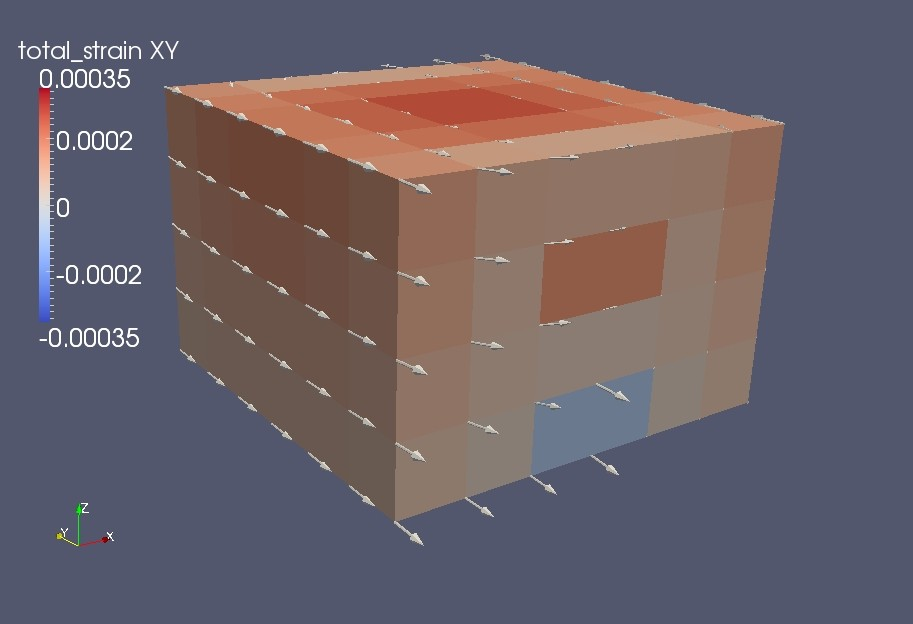
\includegraphics[width=10cm]{examples/figs/3dhex8_step08-strain-displ-t150}
  \caption{The XY-component of strain (color contours) and displacement field
    (vectors) for example step08 at t = 150 years visualized using ParaView.
    For this visualization, we loaded both the \filename{step08-lower\_crust.xmf}
    and \filename{step08-upper\_crust.xmf} files to contour the strain field,
    and superimposed on it the displacement field vectors from \filename{step08.xmf}.}
  \label{fig:example:3dhex8:step8:displacement}
\end{figure}


\subsubsection{Step09 - Dirichlet Velocity Boundary Conditions with Time-Dependent
Kinematic Fault Slip and Drucker-Prager Elastoplastic Rheology}

In this example we use a Drucker-Prager elastoplastic rheology in
the lower crust. As in example step08, the material behavior is nonlinear
so we again use the nonlinear solver. The material is elastoplastic,
there is no inherent time-dependent response and the stable time-step
size for the material depends on the loading conditions. To avoid
this, we set the maximum time-step size to 5 years rather than the
value of 10 years used in example \filename{step08}:
\begin{cfg}[Excerpt from \filename{step09.cfg}]
# Change the total simulation time to 700 years, and set the maximum time
# step size to 5 years.
<h>[pylithapp.timedependent.implicit.time_step]</h>
<p>total_time</p> = 700.0*year
<p>max_dt</p> = 5.0*year
<p>stability_factor</p> = 1.0 ; use time step equal to stable value from materials

# For this problem we set adapt\_skip to zero so that the time step size is
# readjusted every time step.
<p>adapt_skip</p> = 0

# Change material type of lower crust to Drucker-Prager.
<h>[pylithapp.timedependent]</h>
<f>materials.lower_crust</f> = pylith.materials.DruckerPrager3D

# Provide a spatial database from which to obtain property values.
# In this case, we prefer to obtain the Drucker-Prager properties from one
# database and the elastic properties from another database, so we use
# a CompositeDB. Each part of the CompositeDB is a SimpleDB.
<h>[pylithapp.timedependent.materials.lower_crust]</h>
<f>db_properties</f> = spatialdata.spatialdb.CompositeDB
<f>db_properties.db_A</f> = spatialdata.spatialdb.SimpleDB
<f>db_properties.db_B</f> = spatialdata.spatialdb.SimpleDB
\end{cfg}
As for the step08 example, we first define the properties that come
from each spatial database and then provide the database filename:
\begin{cfg}[Excerpt from \filename{step09.cfg}]
# Provide the values to be obtained from each database and the database
# name.
<h>[pylithapp.timedependent.materials.lower_crust.db_properties]</h>
<p>values_A</p> = [density,vs,vp] ; Elastic properties.
<p>db_A.label</p> = Elastic properties
<p>db_A.iohandler.filename</p> = spatialdb/mat_elastic.spatialdb

<p>values_B</p> = [friction-angle, cohesion, dilatation-angle] ; Drucker-Prager properties.
<p>db_B.label</p> = Drucker-Prager properties
<p>db_B.iohandler.filename</p> = spatialdb/mat\_druckerprager.spatialdb
\end{cfg}
We also request output of the properties and state variables that
are unique to the \object{DruckerPrager3D} material:
\begin{cfg}[Excerpt from \filename{step09.cfg}]
# Since there are additional properties and state variables for the
# Drucker-Prager model, we explicitly request that they be output.
# Properties are named in cell\_info\_fields and state variables are named in
# cell_data_fields.
<h>[pylithapp.timedependent.materials.lower_crust]</h>
<p>output.cell_info_fields</p> = [density, mu, lambda, alpha_yield, beta, alpha_flow]
<p>output.cell_data_fields</p> = [total_strain, stress, plastic_strain]
\end{cfg}
When we have run the simulation, the output HDF5 and Xdmf files will
be contained in \filename{examples/3d/hex8/output} (all with a prefix
of \filename{step09}). Results using ParaView are shown in Figure
\vref{fig:example:3dhex8:step09:displacement}.

\begin{figure}
  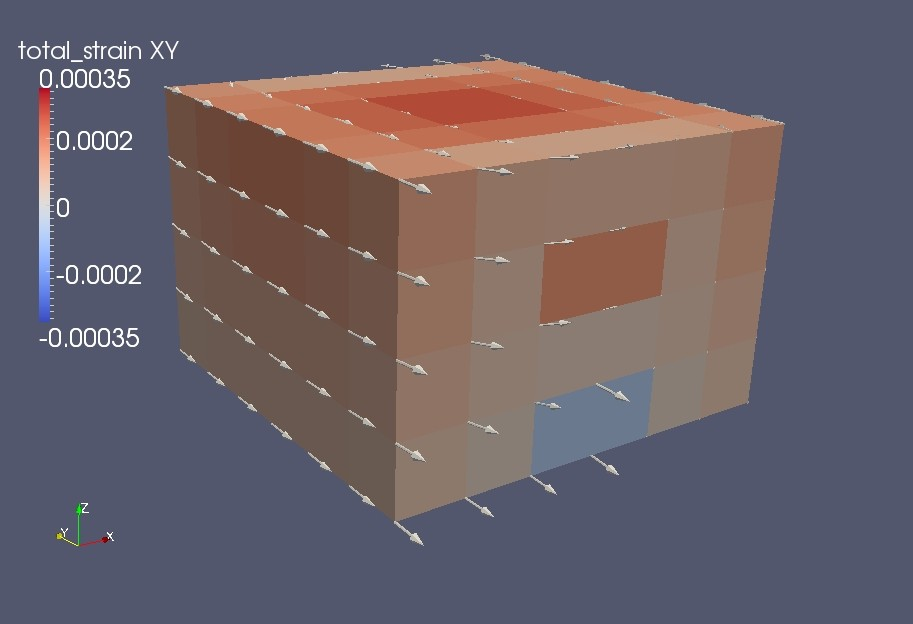
\includegraphics[width=10cm]{examples/figs/3dhex8_step08-strain-displ-t150}
  \caption{The XY-component of strain (color contours) and displacement field
    (vectors) for example step09 at t = 150 years visualized using ParaView.
    For this visualization, we loaded both the \filename{step09-lower\_crust.xmf}
    and \filename{step09-upper\_crust.xmf} files to contour the strain field,
    and superimposed on it the displacement field vectors from \filename{step09.xmf}.}
  \label{fig:example:3dhex8:step09:displacement}
\end{figure}

% End of file
